\documentclass[letter]{IEEEtran}

\usepackage{amsmath}
\usepackage{amssymb}
\usepackage{graphicx}
\usepackage{algorithmic}
\usepackage{algorithm}
\usepackage{flushend}

\DeclareGraphicsExtensions{.pdf,.jpeg,.png,.jpg, .eps}
\graphicspath{{images/}}

\title{EKF: Attitude}
\date{\today}
\begin{document}
\author{Luke Fraser}
\maketitle

\begin{abstract}
In this assignment we investigate the use of an EKF to estimate the attitude of an IMU. We model the attitude of the sensor and estimate the sensor state of real IMU data from a \emph{rosbag} file. Extending the Kalman filter to handle non-linear sensor models. The data is then plotted against the actual IMU raw data and compared against the estimated attitude.
\end{abstract}

\section{Introduction}
\subsection{Kalman Filter}
remely useful tool for estimating noisy variables in a system. Its uses stretch far beyond uses in drone state estimation. It can be used within an IMU, as a tracker for computer vision, reading temperature readings, etc. Kalman filter uses extent into many domains. As a basic kalman filter is a linear estimator it is very fast and simple to use and implement making it perfect for different applications. Although the Kalman filter is a very capable estimator its simplicity limits is capabilities.

The Kalman filter due to its assumption of linearity it is only meant handle estimation of variable that abide by this assumption. In the case of state estimation of a quad-rotor pose in $\mathbb{R}^3$ the kalman filter does not perform as well. This is due to the non-linearity of the state of the drone. To fix this problem the extended kalman filter (EKF) was created to handle the non-linear nature of real-world state estimation problems.

Today EKF's are used to solve many complex estimation problems in real-time. A more simple alternative to drones is the estimation of a car. As the degrees of freedom are smaller EKF performance on cars has been well tuned and can be used to help produce self-driving cars.

\subsection{Extended Kalman Filter}
\begin{equation}
\label{eq:kfstatemodel}
x_k = Ax_{k-1} + Bu_{k}
\end{equation}
The EKF extends the KF to handle non-linear state models. In this way the model equation~\ref{eq:kfstatemodel} is replaced by a non-linear function $g(x_{t-1}, u_t)$ as seen in equation~\ref{eq:statemodel}. This brakes the requirement that the state transiftions are linear.
\begin{equation}
\label{eq:statemodel}
x_t = g(x_{t-1}, u_t) + w_t
\end{equation}
\begin{equation}
\label{eq:kfmeasuremodel}
z_t = H_t x_t + v_k
\end{equation}
The measurement model for the KF is a linear fuction of the measurement data as shown in equation~\ref{eq:kfmeasuremodel}. This equation provides the linear measure transiftion function for the kalman filter. The EKF extends this model to not assume a linear model. Equation~\ref{eq:measure_model} shows the non-linear equation defining the measure transistion function.
\begin{equation}
\label{eq:measure_model}
z_t = h(x_t) + v_k
\end{equation}

These equations are used to model the state estimate in the EKF algortihm. The two steps of the EKF algirithm are show in algorithms~\ref{alg:predict},~\ref{alg:correct}. These two steps form the complete EKF algorithm.
\begin{algorithm}
\caption{EKF - Prediction Step}
\begin{algorithmic}[1]
\STATE $\bar{x_t} = g(x_{t-1}, u_t)$
\STATE $\bar{P_t} = G_t P_{t-1} G_t^T + R_t$
\end{algorithmic}
\label{alg:predict}
\end{algorithm}

The EKF prediction step like the prediction step of the KF predicts the state based on the precious state estimate. This is an important step of the EKF as it predicts based on the non-linear transition function that models the state change. In the case of estimate mating the attitude of the drone a model is used that integrates the angular rates to acquire the attitude of the IMU.
\begin{equation}
\label{eq:model}
x_t = 
\begin{bmatrix}
  \dot{\phi}_{t} \\
  \dot{\theta}_{t}\\
  \dot{\psi}_{t}\\
  \phi_{t}\\
  \theta_{t}\\
  \psi_{t}\\
\end{bmatrix}
= g(x_{t-1}, u_t) =
\begin{bmatrix}
  \dot{\phi}_{t-1} \\
  \dot{\theta}_{t-1}\\
  \dot{\psi}_{t-1}\\
  \phi_{t-1} + \dot{\phi}_{t-1} dt\\
  \theta_{t-1} + \dot{\theta}_{t-1} dt\\
  \psi_{t-1} + \dot{\psi}_{t-1} dt\\
\end{bmatrix}
\end{equation}
Equation~\ref{eq:model} shows the transition model of the state vector. This model is used to perform the prediction udpate as shown in \ref{alg:predict}. This is the crucial model that defines the state of the attitude of the IMU. The model itself is very simple. The angular velocites are simply assumed to stay the same between each prediction step as there is no information that would infer a change in the model. An addition that would help predict the angular velocities ($\dot\phi,~\dot\theta,~\dot\psi$) would be a GPS unit. This would allow a more complex transition function based on the previous position estimated.

The main state estimate that is acheived from this model is integrating to compute the angles of IMU ($\phi,~\theta,~\psi$). This makes sense as to predict the next state we take the angular rate and integrate of the time since the last reading and add it to the current estimate of the attitude. This will produce the predicted state of the IMU.

\begin{algorithm}
\caption{EKF - Correction Step}
\begin{algorithmic}[1]
\STATE $K_t = P_t H_t^T (H_t P_t H_t^T + Q_t)^{-1}$
\STATE $x_t = \bar{x_t} + K_t (z_t - h(\bar{x_t}))$
\STATE $P_t = (I - K_t H) \bar{P_t}$
\end{algorithmic}
\label{alg:correct}
\end{algorithm}

The correction step of the EKF just like the KF has very similar structure. The main differences are the non-linear transistion Joacobians and funtions. $G_t$ and $H_t$ are the transition jacobians of the state prediction and the measurement. These matrices are used to linearize the non-linear model of the EKF. In this way the EKF is able to handle the non-linear model provided. Due to the simple nature of the model in question the jocobian of $g$ and $h$ are shown in equations~\ref{eq:gjacobian},~\ref{eq:hjacobian}.

\begin{equation}
\label{eq:gjacobian}
G_t = 
\begin{bmatrix}
1 & 0 & 0 & 0 & 0 & 0 \\
0 & 1 & 0 & 0 & 0 & 0 \\
0 & 0 & 1 & 0 & 0 & 0 \\
dt& 0 & 0 & 1 & 0 & 0 \\
0 & dt& 0 & 0 & 1 & 0 \\
0 & 0 & dt& 0 & 0 & 1 \\
\end{bmatrix}
\end{equation}
\begin{equation}
\label{eq:hjacobian}
H_t = 
\begin{bmatrix}
1 & 0 & 0 & 0 & 0 & 0 \\
0 & 1 & 0 & 0 & 0 & 0 \\
0 & 0 & 1 & 0 & 0 & 0 \\
\end{bmatrix}
\end{equation}

\section{Results}
\begin{figure}
\centering
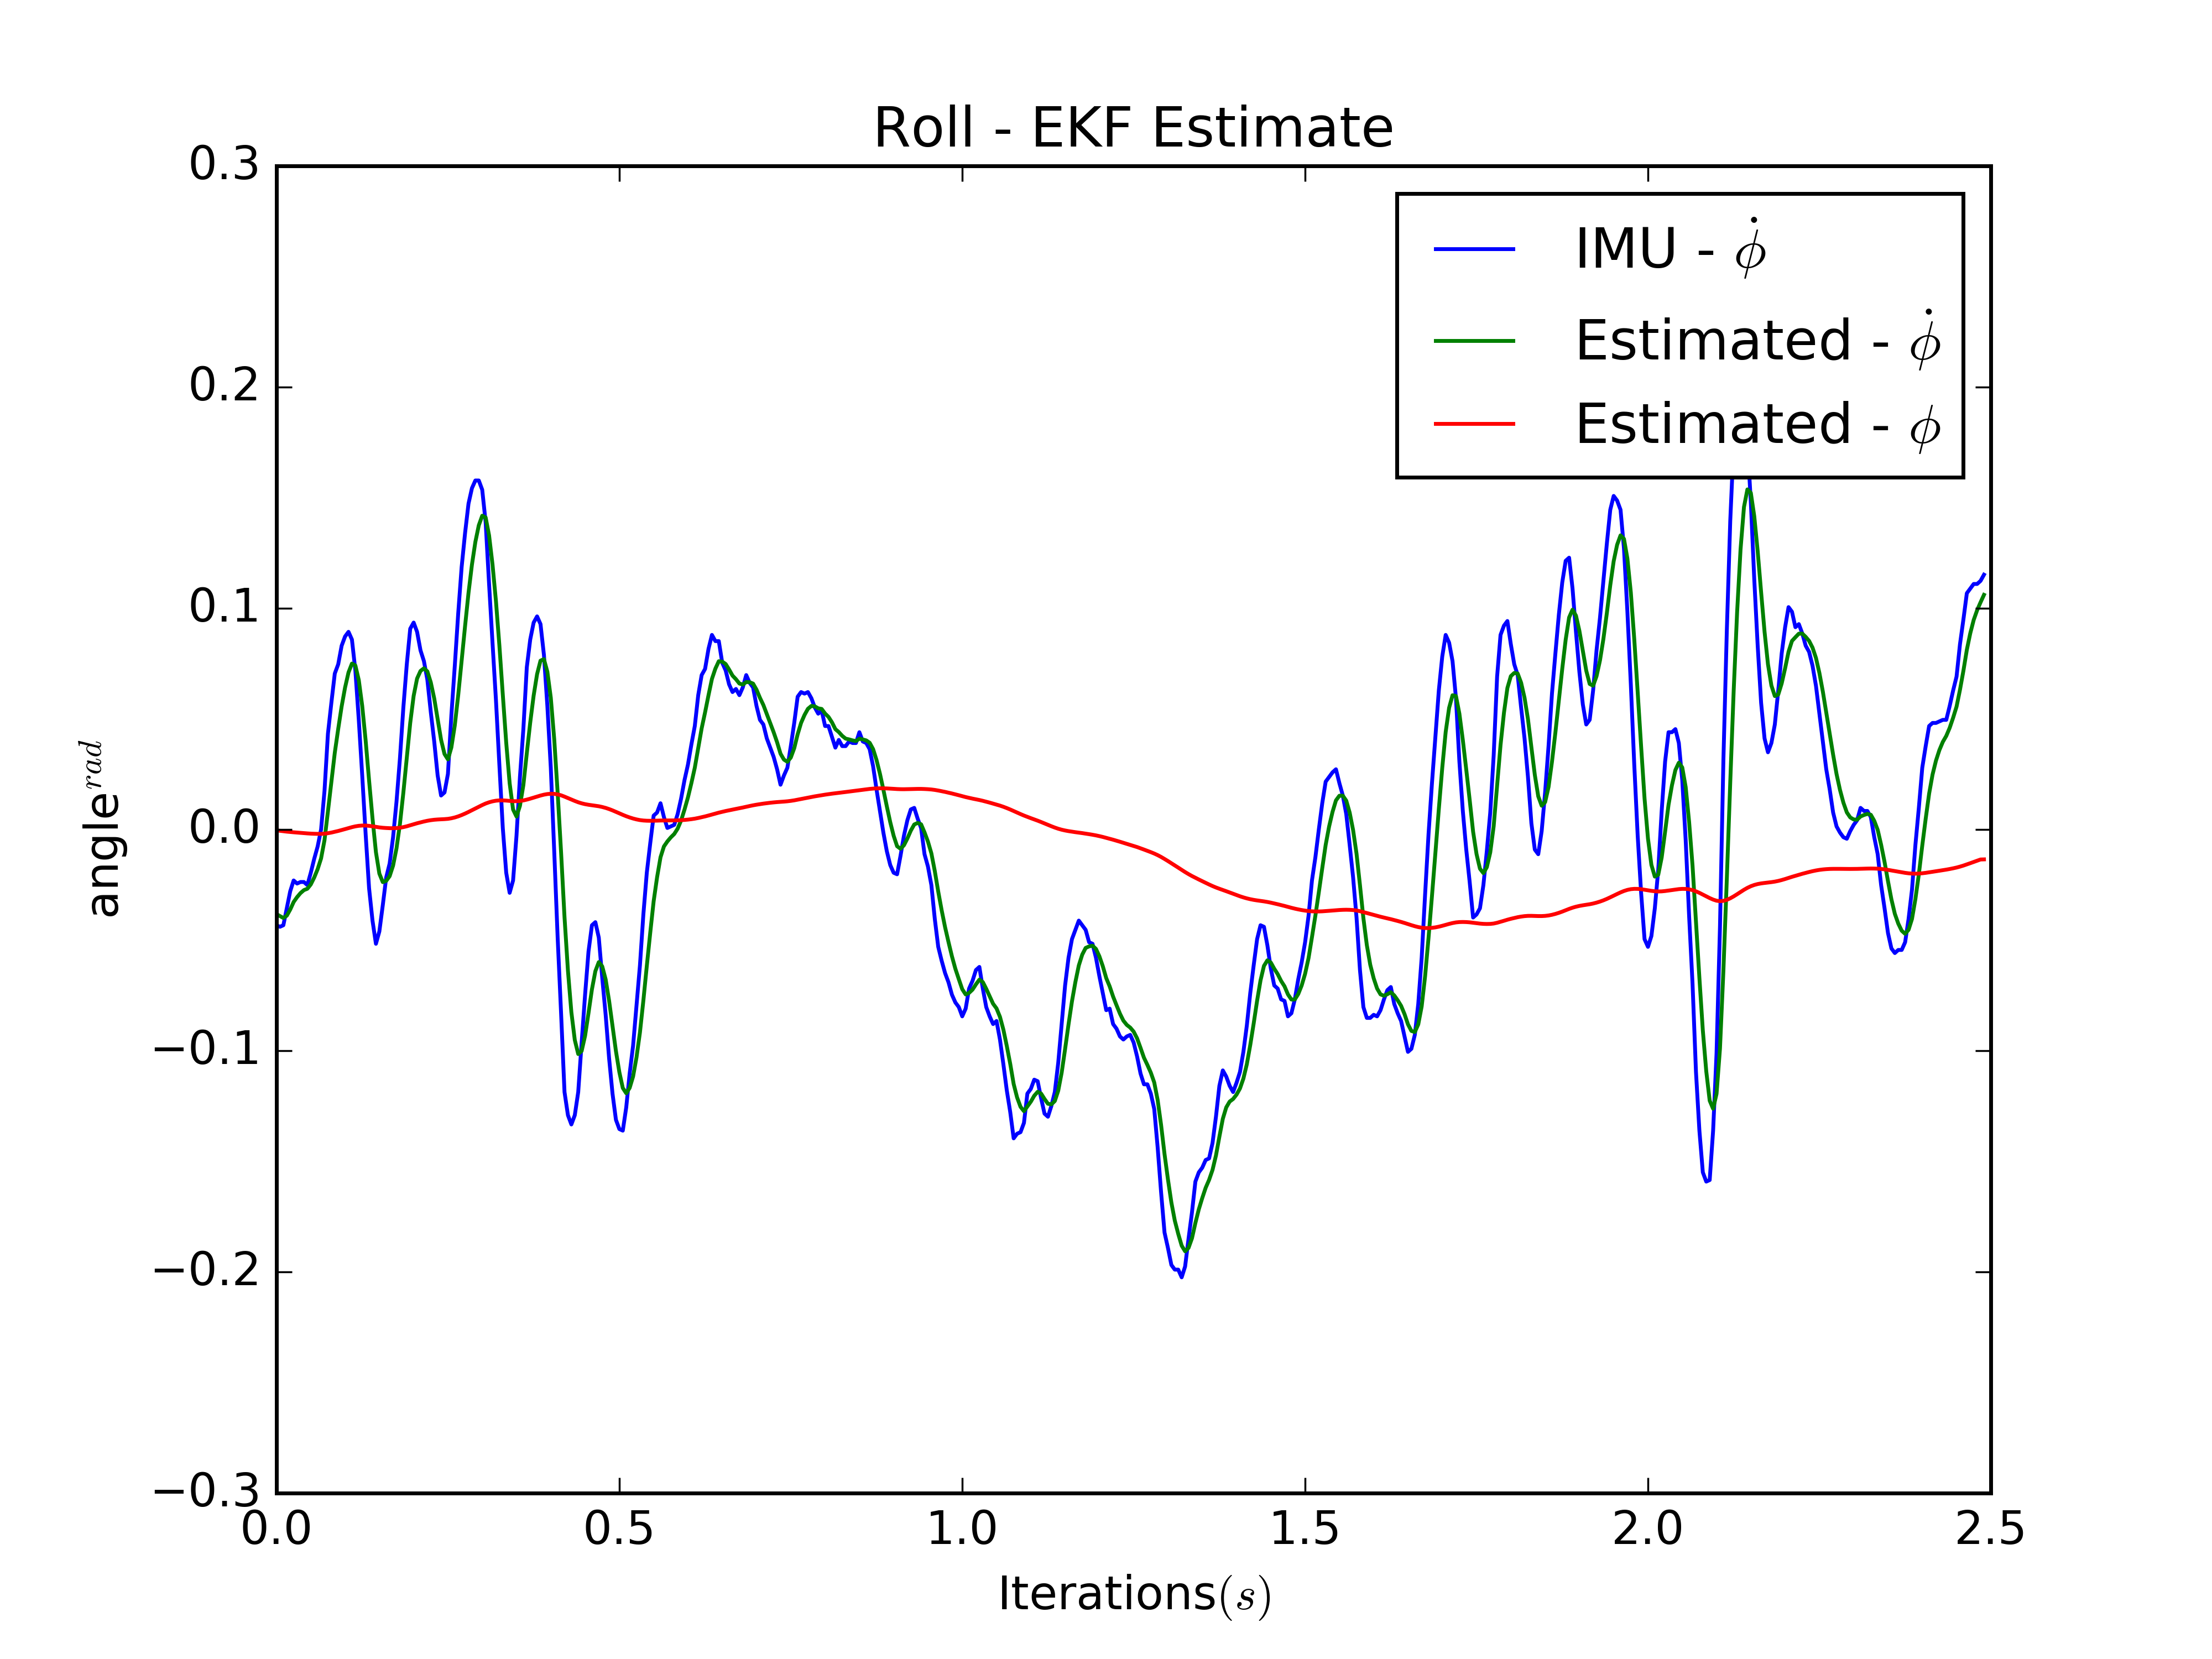
\includegraphics[width=9cm]{roll-result-500-s}
\caption{Roll($\phi$) - Estimation results 500 iterations.}
\label{fig:result-500-roll}
\end{figure}

\begin{figure}
\centering
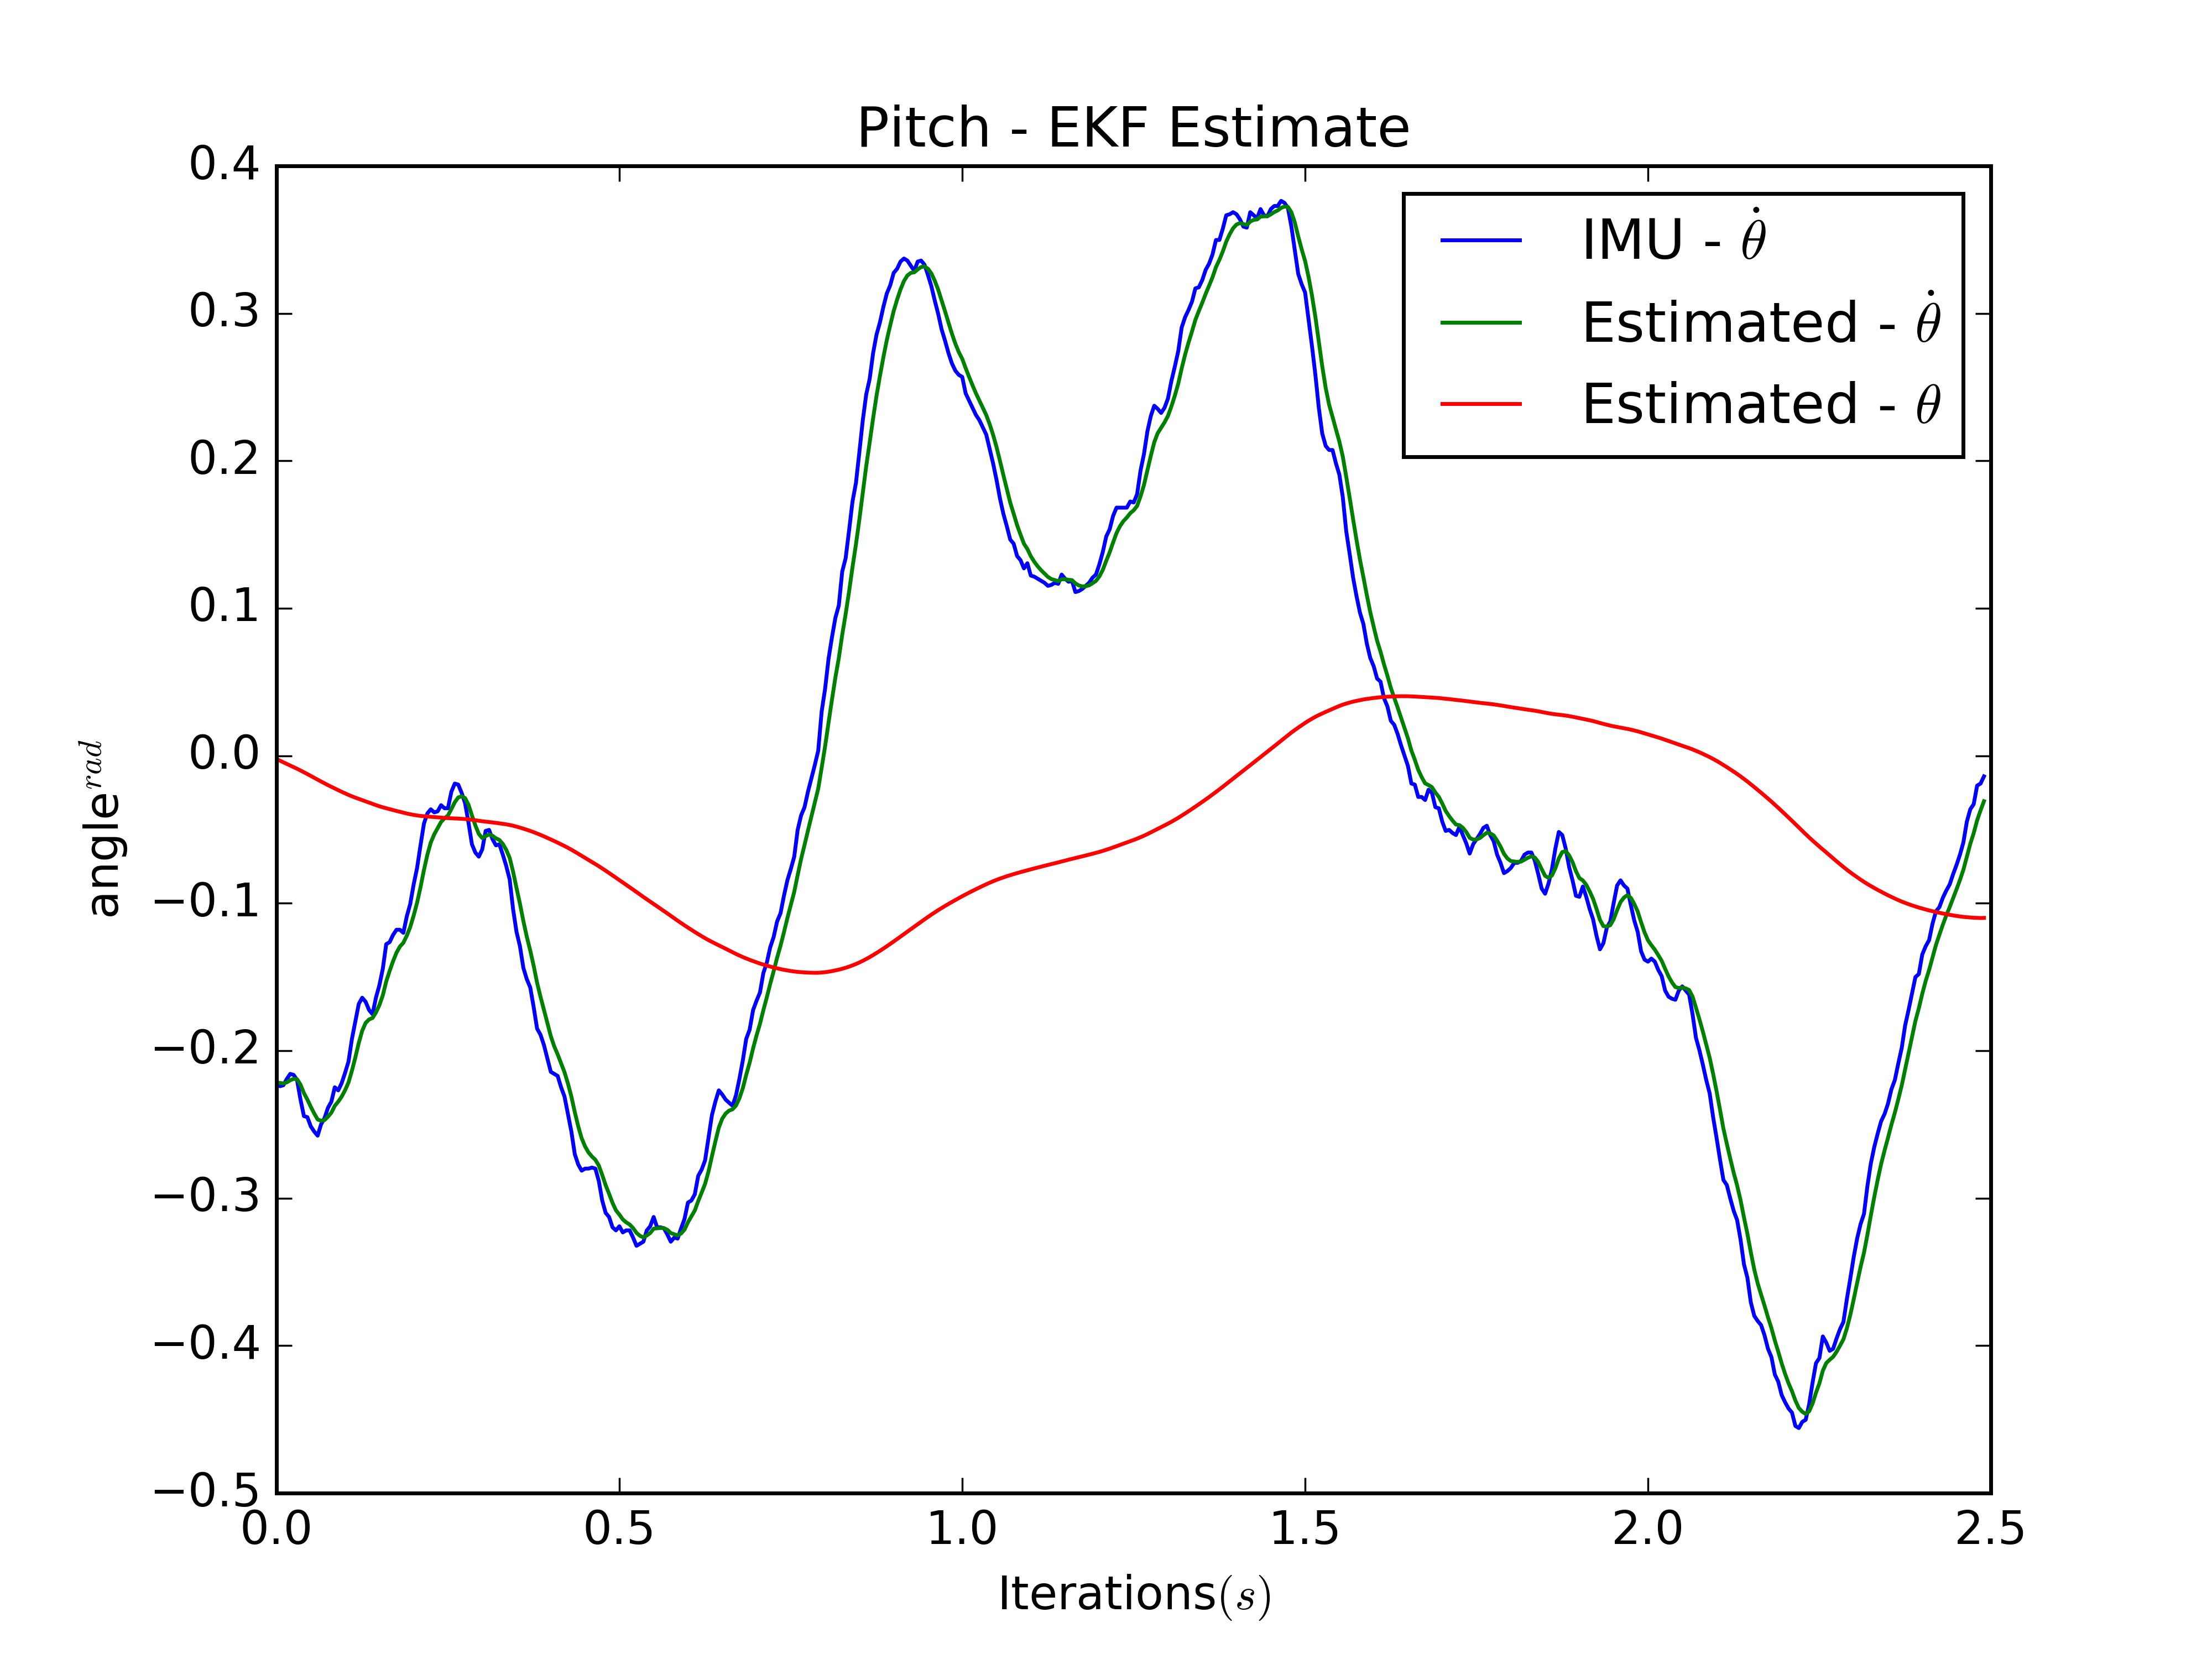
\includegraphics[width=9cm]{pitch-result-500-s}
\caption{Pitch($\theta$) - Estimation results 500 iterations.}
\label{fig:result-500-pitch}
\end{figure}

\begin{figure}
\centering
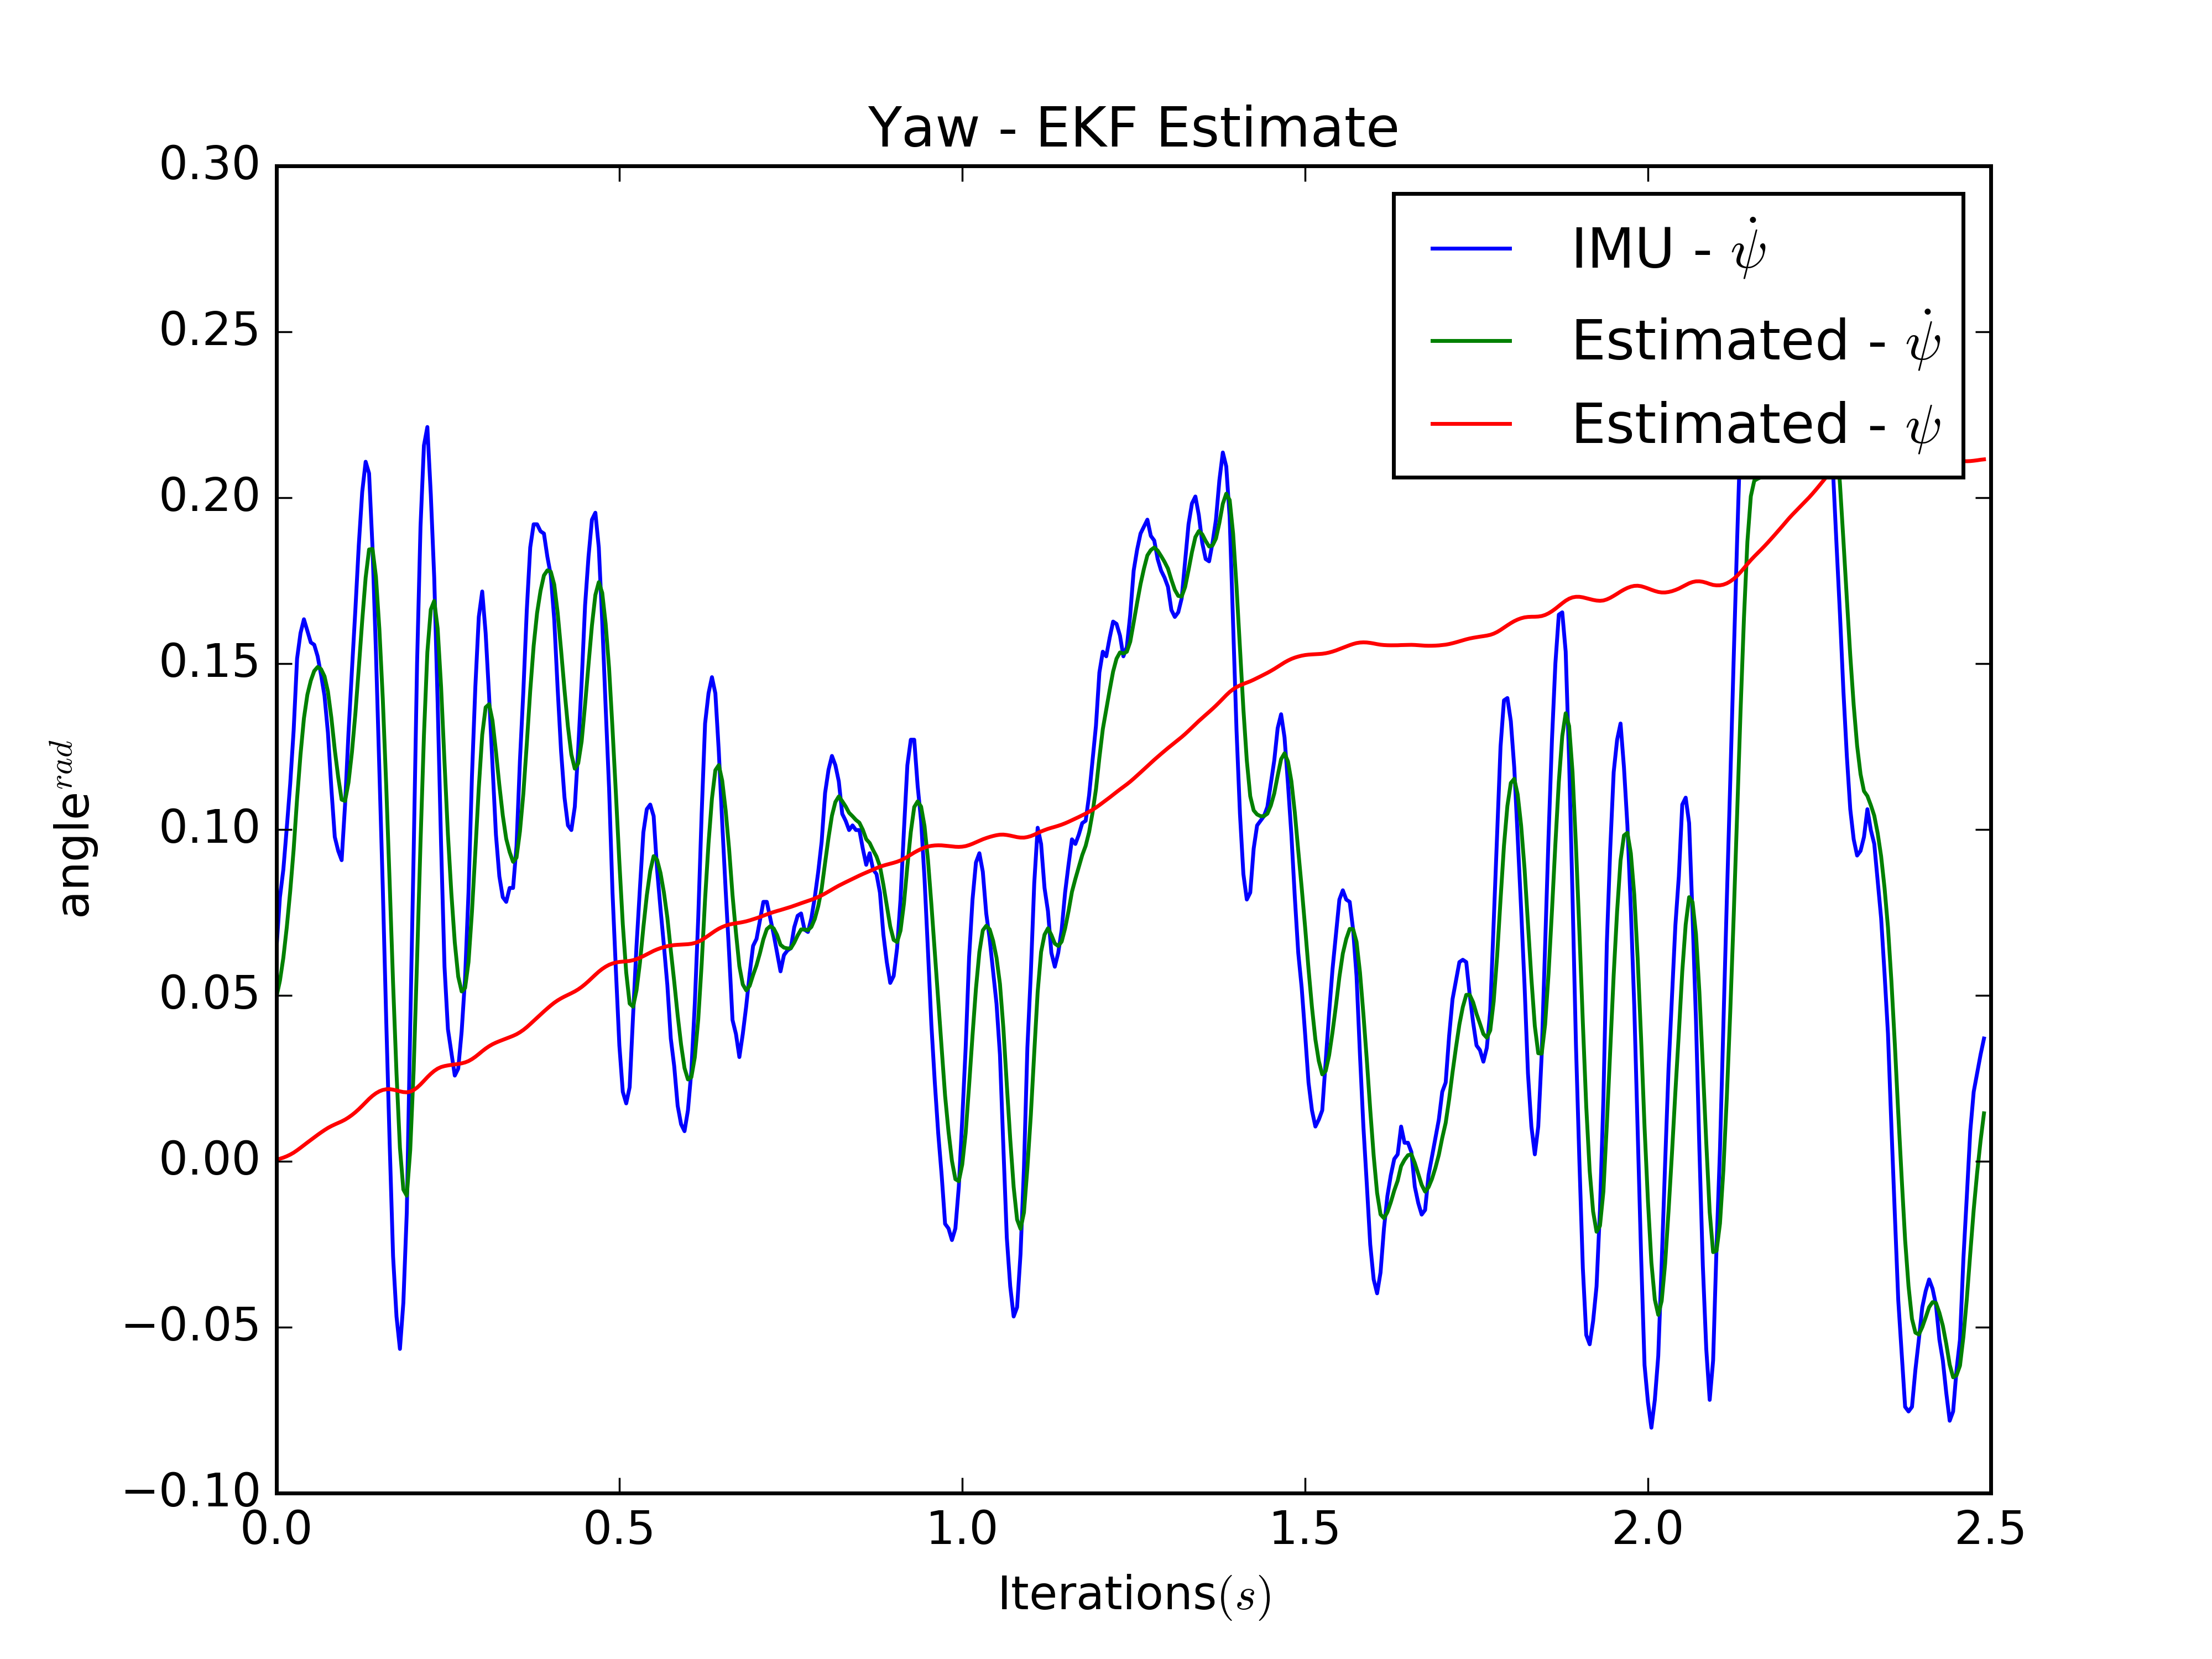
\includegraphics[width=9cm]{yaw-result-500-s}
\caption{Yaw($\psi$) - Estimation results 500 iterations.}
\label{fig:result-500-yaw}
\end{figure}

The results show the EKF algorithm presented above operating on IMU data through a \emph{RosBag} file. Figures~\ref{fig:result-500-roll}, \ref{fig:result-500-pitch}, \ref{fig:result-500-yaw} show the results of filtering 500 frames from the beginning of the \emph{RosBag} file.

\begin{figure}
\centering
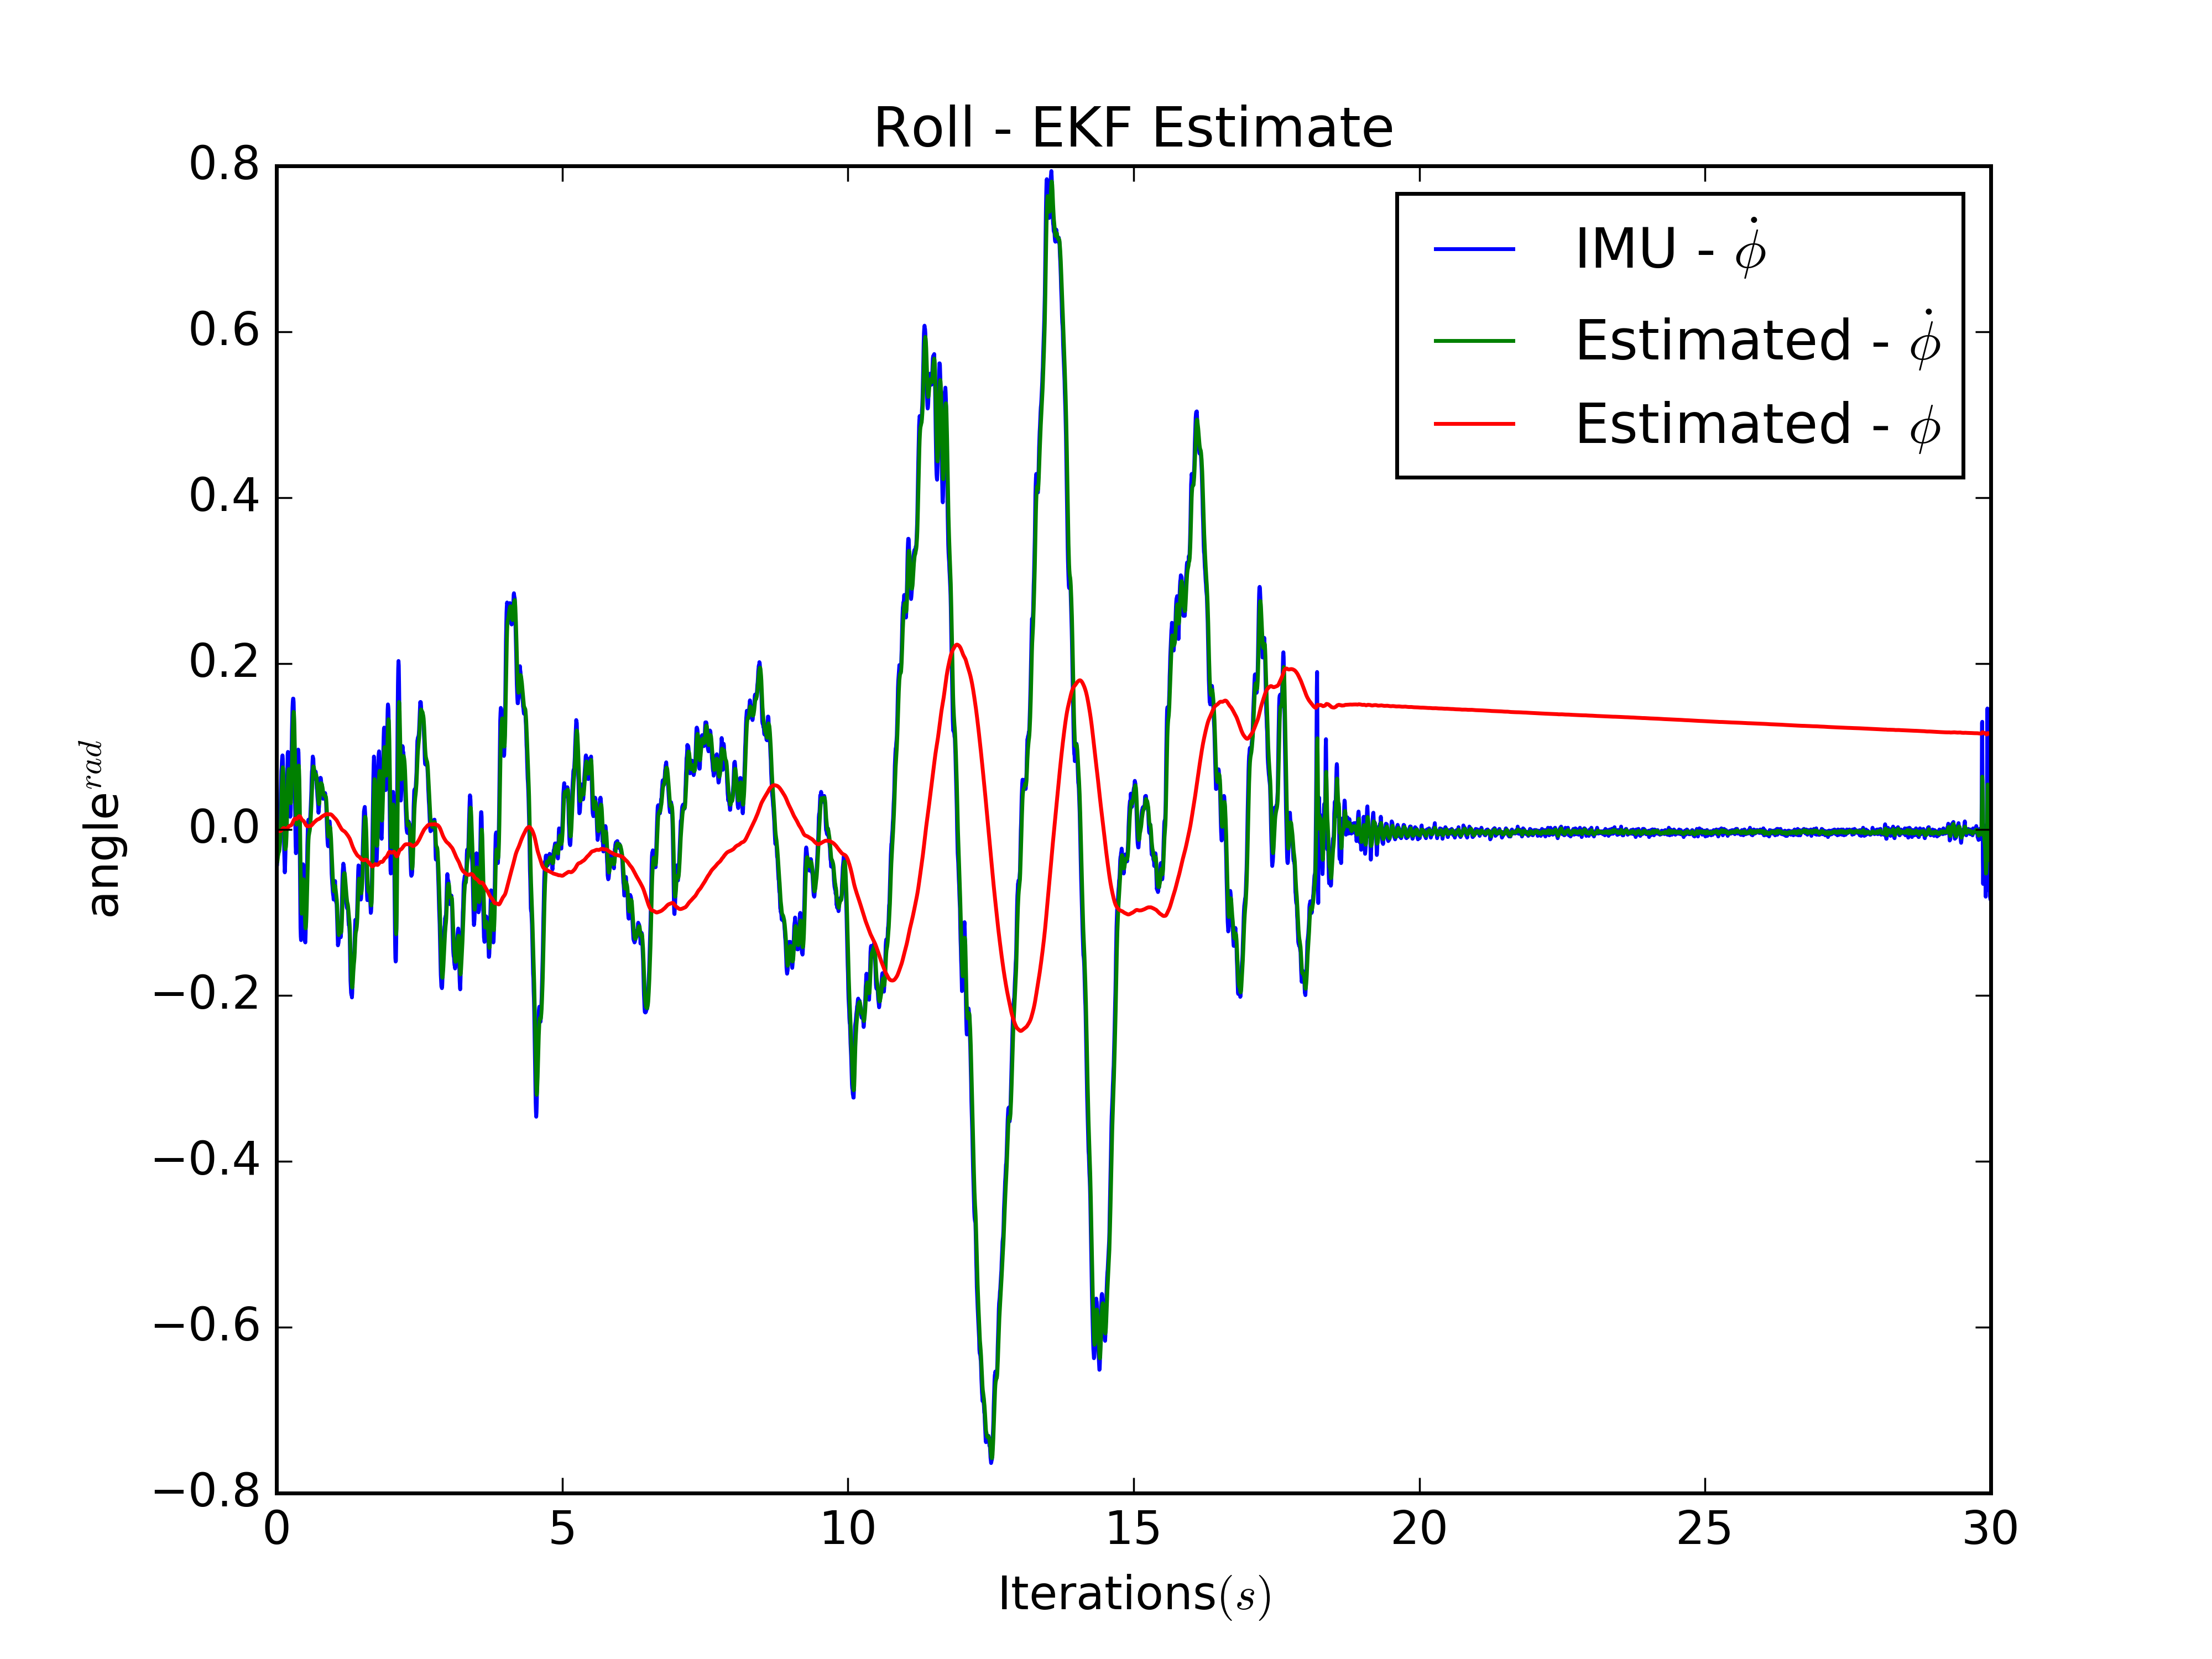
\includegraphics[width=9cm]{roll-result-6000-s}
\caption{Roll($\phi$) - Estimation results 6000 iterations.}
\label{fig:result-6000-roll}
\end{figure}

\begin{figure}
\centering
  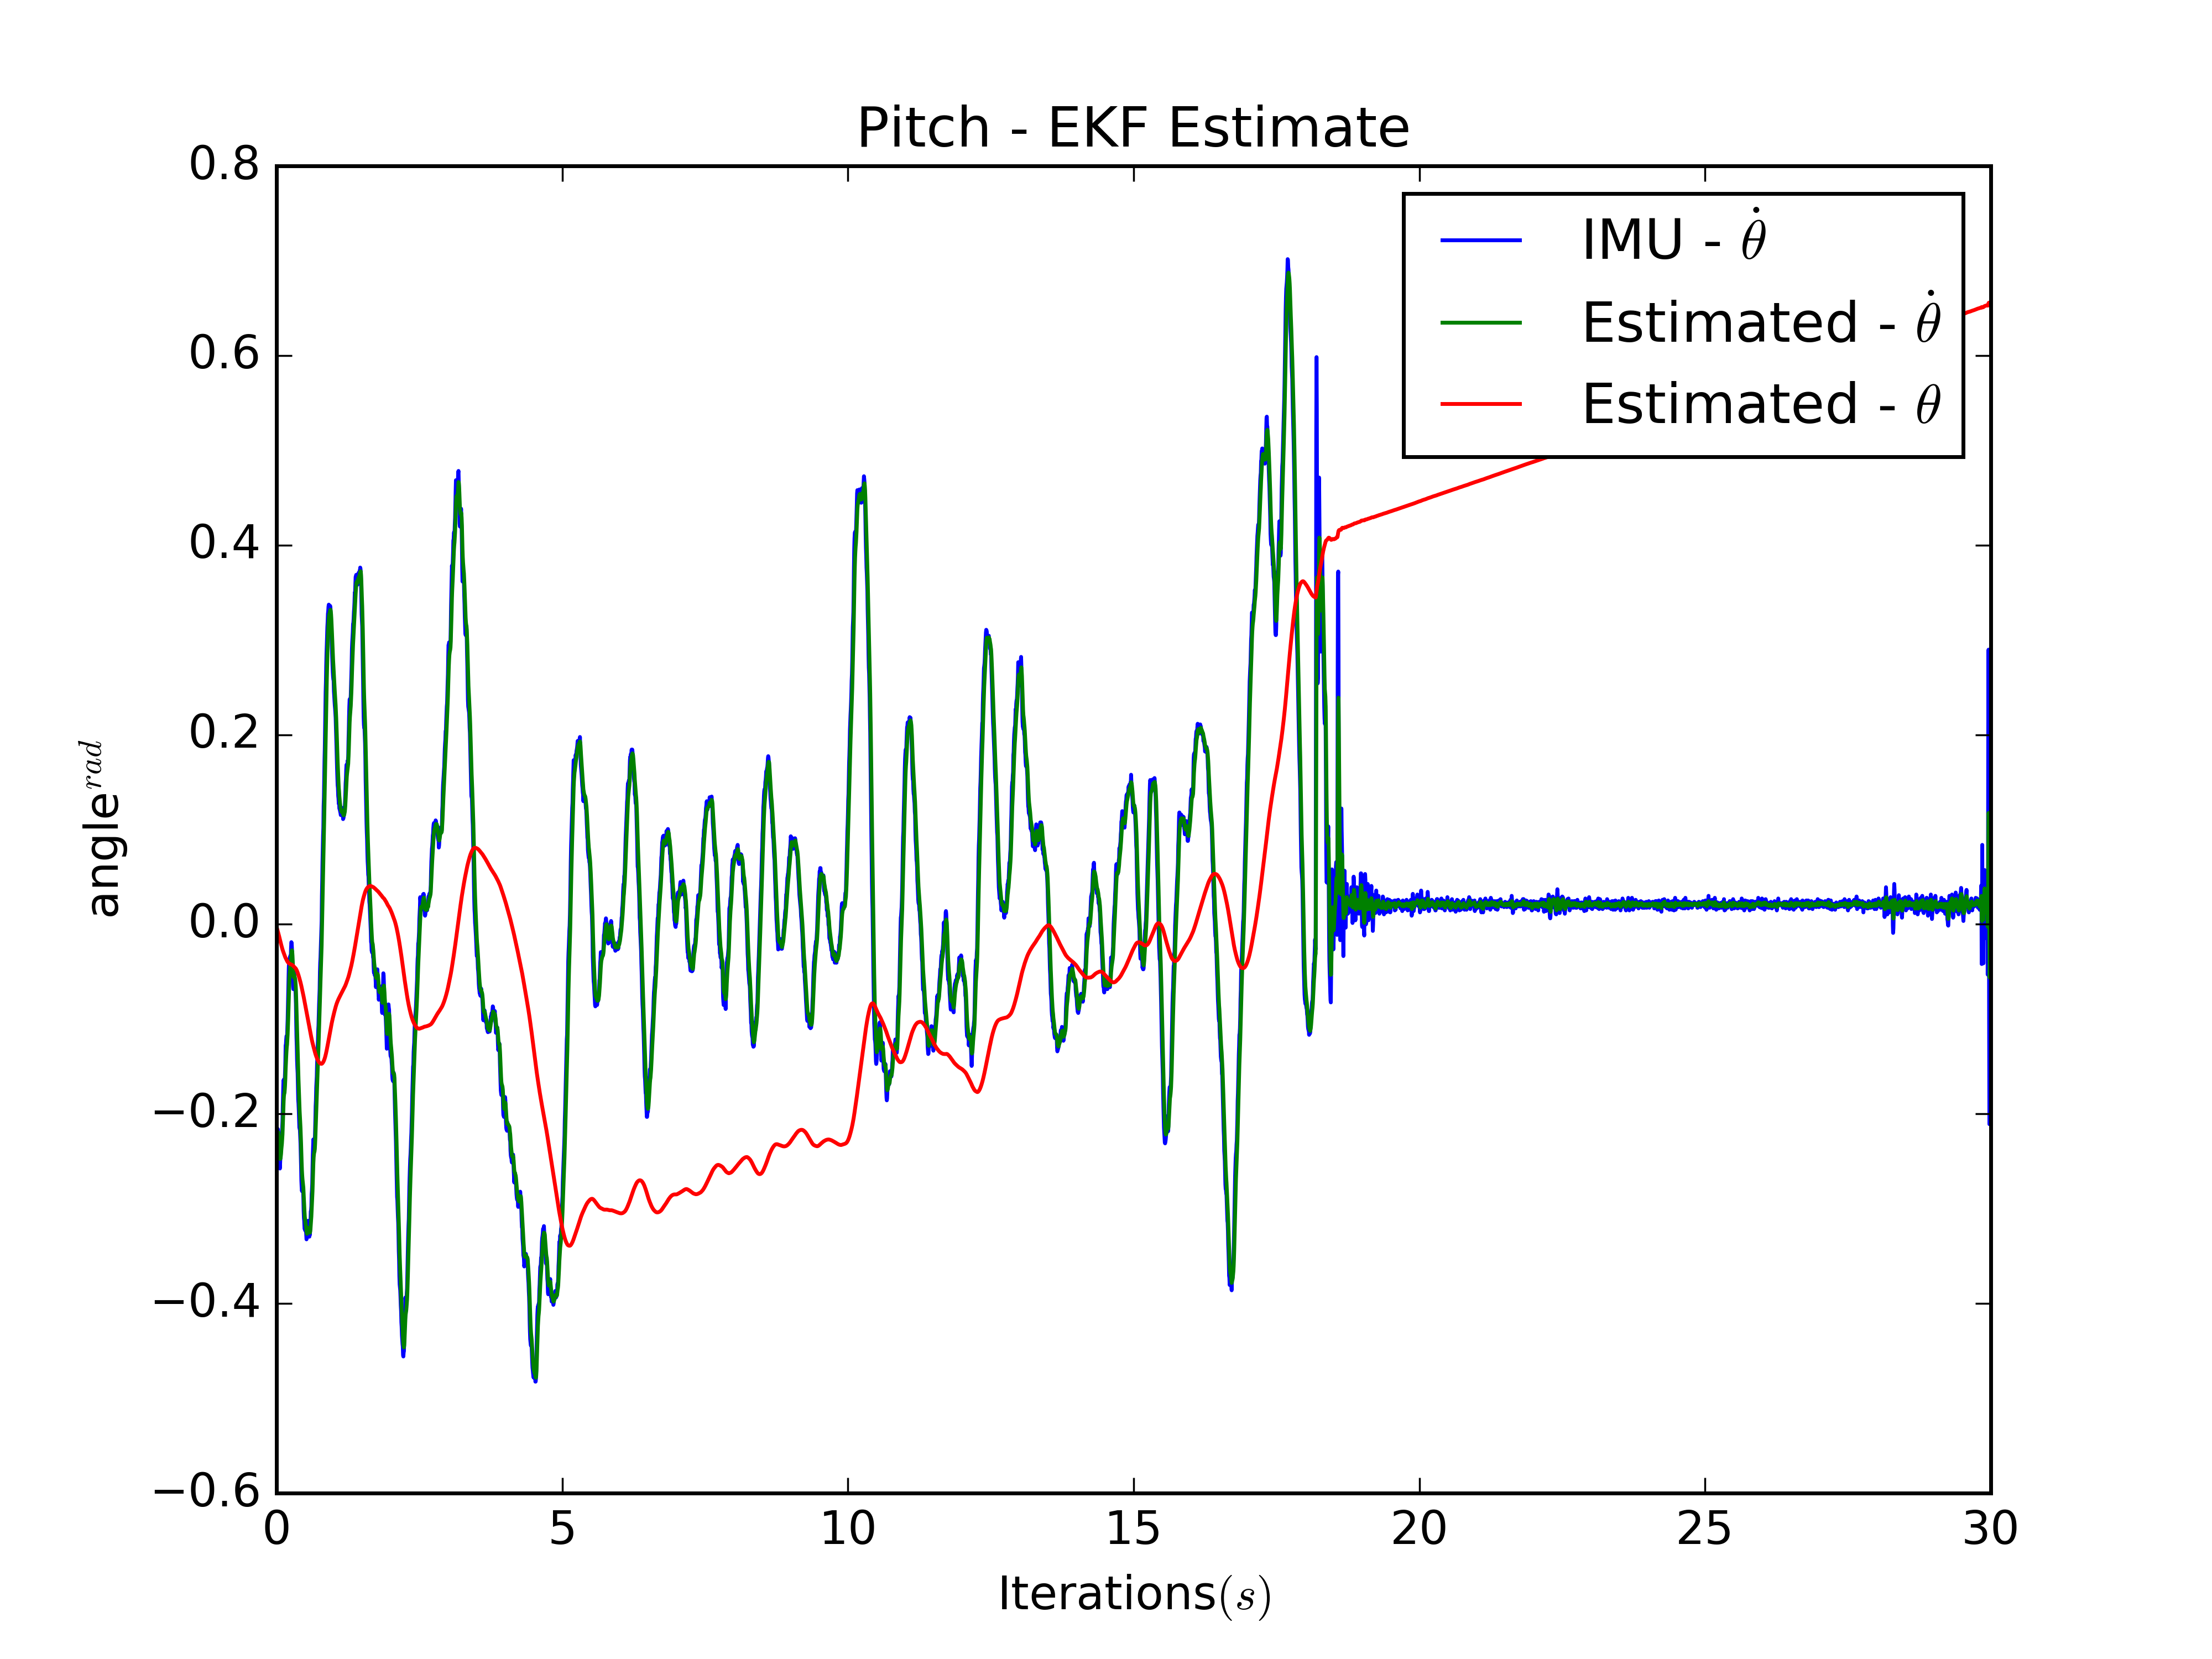
\includegraphics[width=9cm]{pitch-result-6000-s}
\caption{Pitch($\theta$) - Estimation results 6000 iterations.}
\label{fig:result-6000-pitch}
\end{figure}

\begin{figure}
\centering
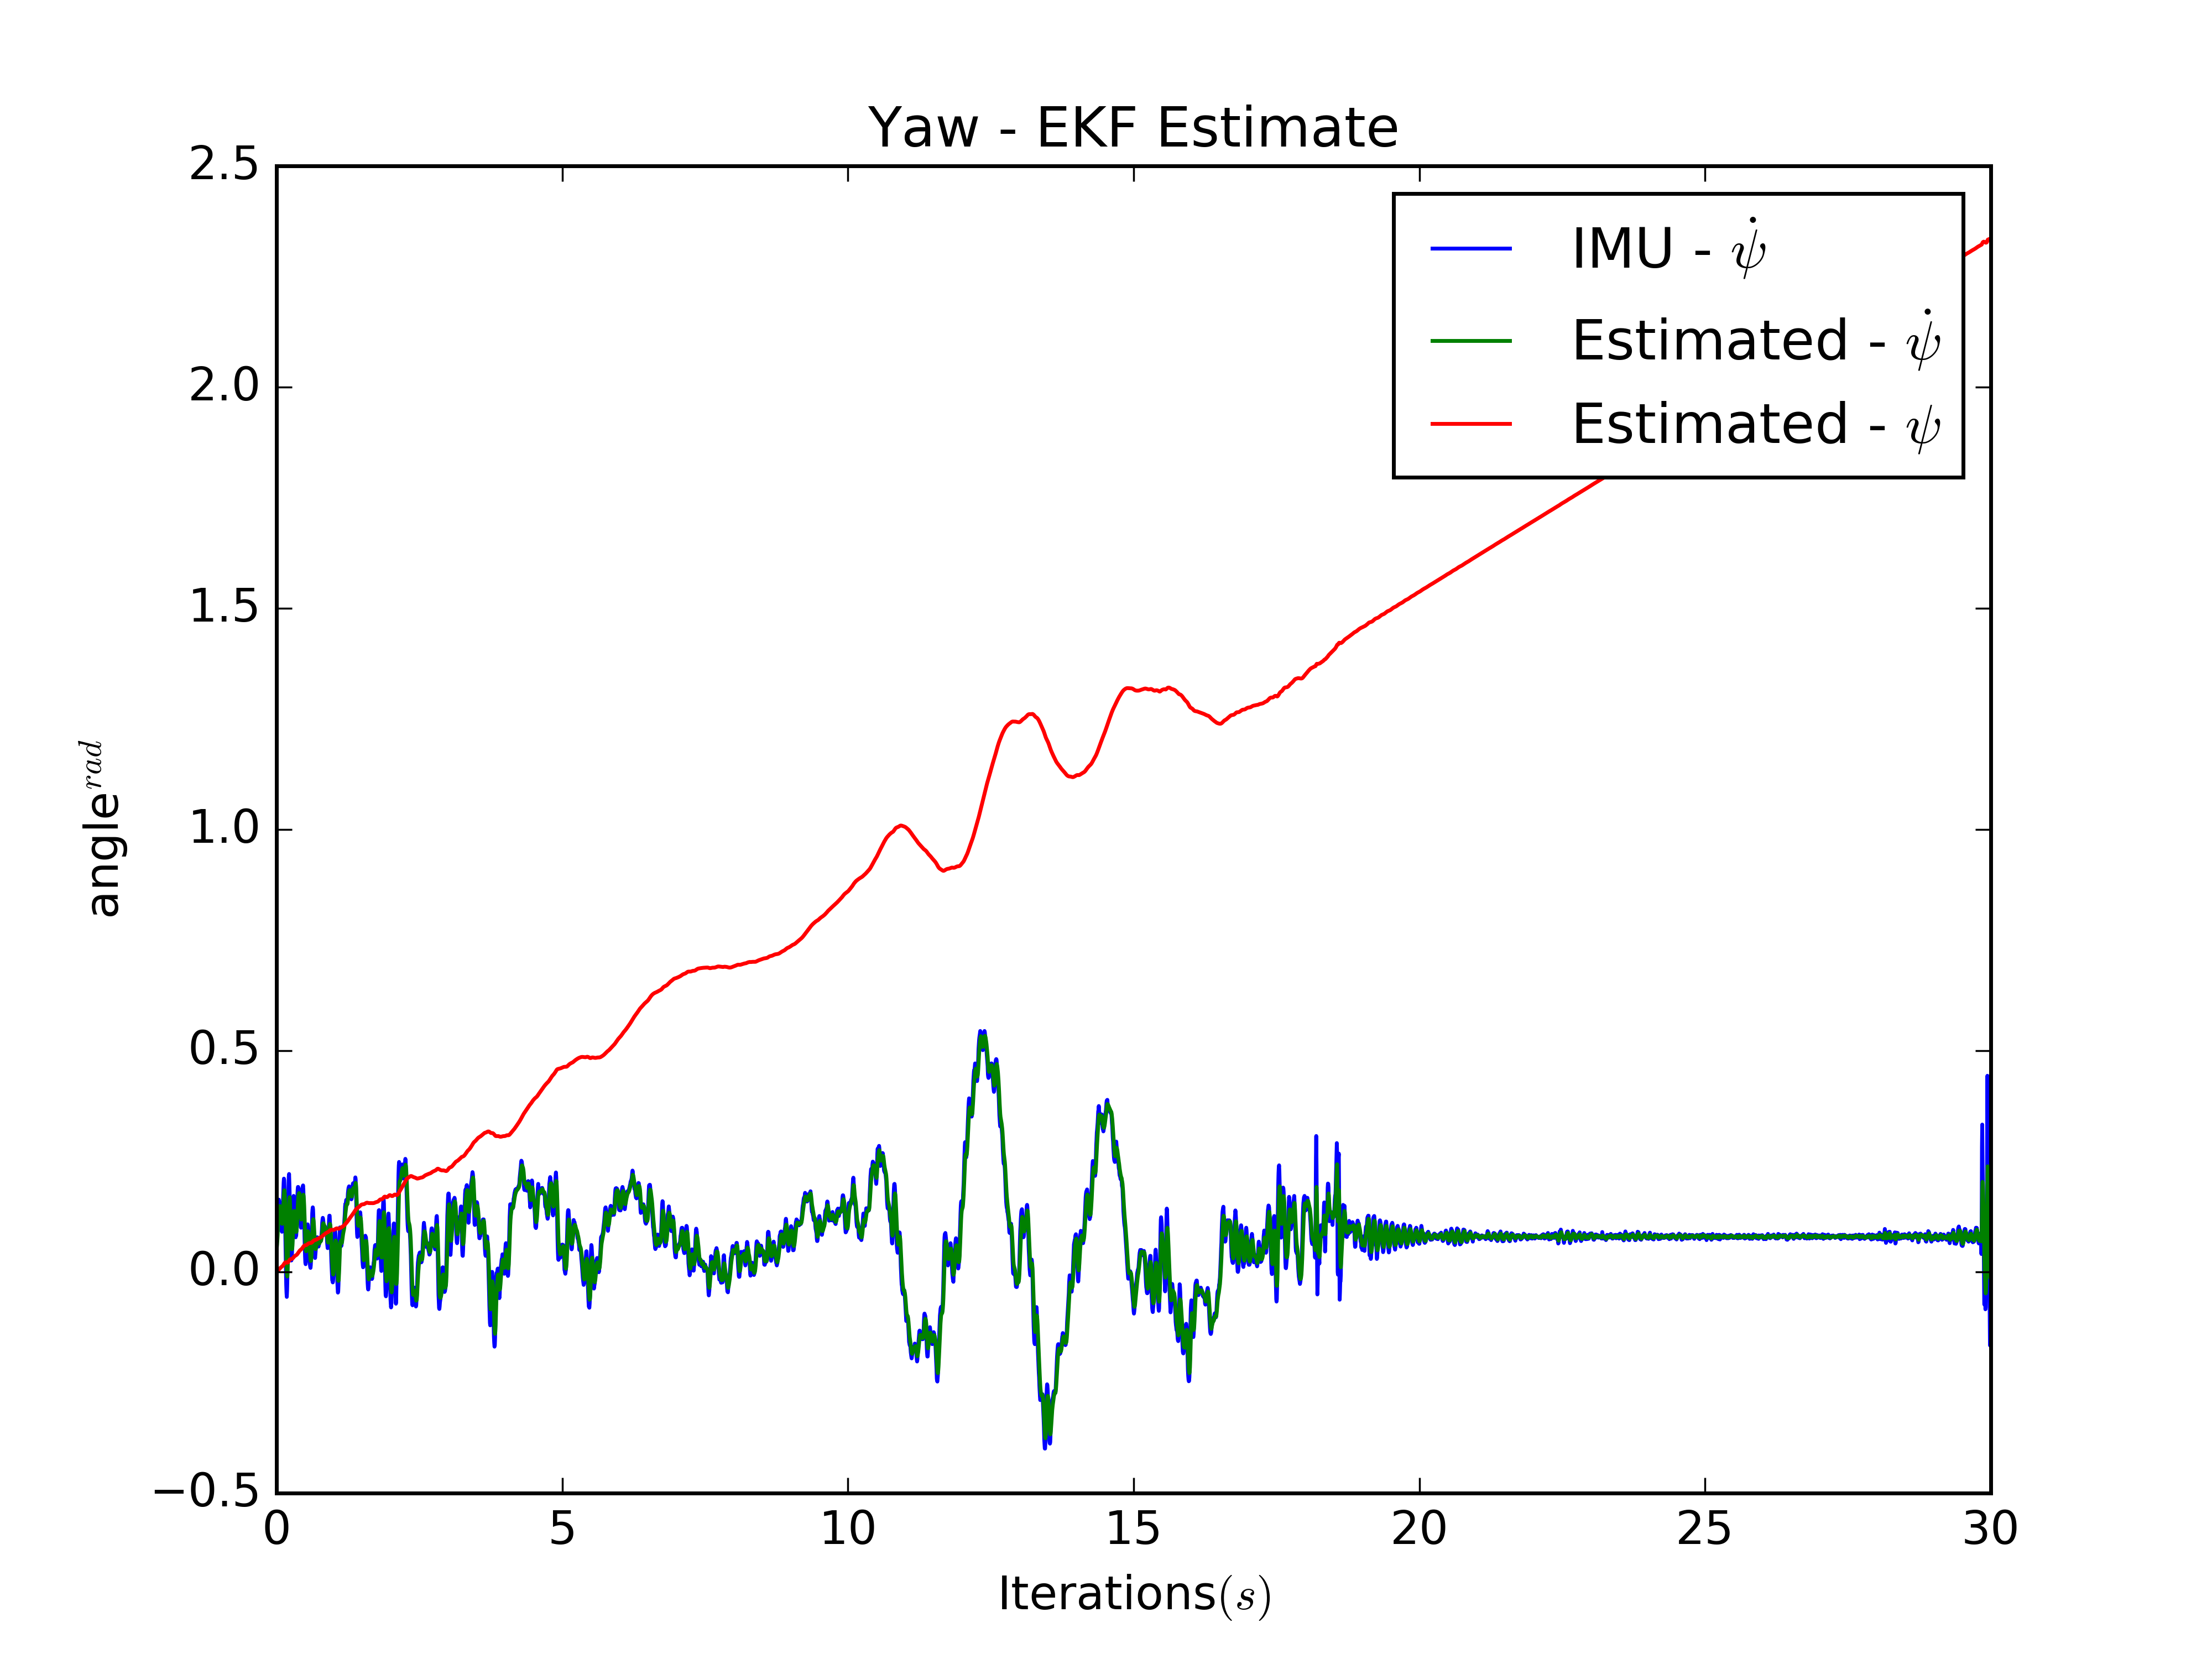
\includegraphics[width=9cm]{yaw-result-6000-s}
\caption{Yaw($\psi$) - Estimation results 6000 iterations.}
\label{fig:result-6000-yaw}
\end{figure}
Figures~\ref{fig:result-6000-roll},\ref{fig:result-6000-pitch}, \ref{fig:result-6000-yaw} show a larger number of iterations. 6000 samples were used to generate the plots. Interesting trends can be seen in the figures. In the case of the yaw and pitch measurement there is a noticeable drift to the IMU. This is most noticeable in the end of the IMU data sequence. In what seems like a stage where the IMU was placed on a table to be still. Instead of zero angular velocity there are constant biases associated with the data. This causes the EKF estimate of the yaw to increase forever instead of remaining stable and unchanged. The EKF is not able to handle such biases. A GPS is required to fix this issue.

The roll estimate has a much smaller bias associated with it. During the time when the other angular velocities are mostly stable the roll seems to be closest to zero without much of a bias term. This is representative of the roll remaining mostly stable at the end of the sequence.

\section{Conclusion}
Implementing the EKF was a good experience understanding the differnet components that improve opon the standard KF. As well developing the model of the attitude of the IMU was a great learning experience understanding the basics of developing an EKF. Althouhg the EKF performs it is however not tuned and this would play a major roll on the accuracy of the estimations. Having a ground truth with the data from a IR-Camera system would provide interesting information on how well the EKF estimates the state of the drone.

It would also be interesting to see how adding the additional IMU infromation into the model would effect the estimate of the IMU.
\end{document}